


In diesem Abschnitt sind aktuell einige Unterlagen eingefügt, die im Rahmen des Projektes eine Relevanz hatten. Vor Abgabe der Projektarbeit, soll dieser Abschnitt überarbeitet, ausgedünnt und ergänzt werden. 

\section{Projektnotizen}

Austausch und Zusammenarbeite erfolgte auf verschiedenen Platformen:
\begin{itemize}
    \item Gezeichnet und Entwürfe wurden meist in Miro erstellt: \url{https://miro.com/app/board/uXjVOdN2haQ=/}. 
    \item Besprechungen erfolgten meist in Teams: \url{https://teams.microsoft.com/l/team/19%3aDoBvOwOIC6WNhsL9kOIYFKNtVftU1yBtcEn_gcyQtcg1%40thread.tacv2/conversations?groupId=850a22ff-34a2-4fe2-a506-f55ac4d595f8&tenantId=b9b6f99a-a243-422d-ab36-f726574c981a}. 
    \item Der gemeinsame Code und die Dokumentation wurden auf Github erstelt: \url{https://github.com/tstsrv-de/tstsrv-de}. 
\end{itemize}

\subsection{Projektbesprechungen}

Stets Sonntags erfolgten Projektbesprechungen. Notizen und Zusammenfassungen davon finden sich hier in fortschreitender, chronologischer Reihenfolge. Ebenso hier entsprechend einsortiert, finden sich Konzeptzeichnungen und Entwürfe aller Art (UI, Code, Datenbankmodelle).

(TODO!) Bildbeschreibungen ergänzen, wichtige Bilder beschreiben.

2021-11-23-erster-entwurf-gameloop 
\begin{figure}[H]
    \centering
    \caption[]{2021-11-23-erster-entwurf-gameloop}
    \label{fig:2021-11-23-erster-entwurf-gameloop}
    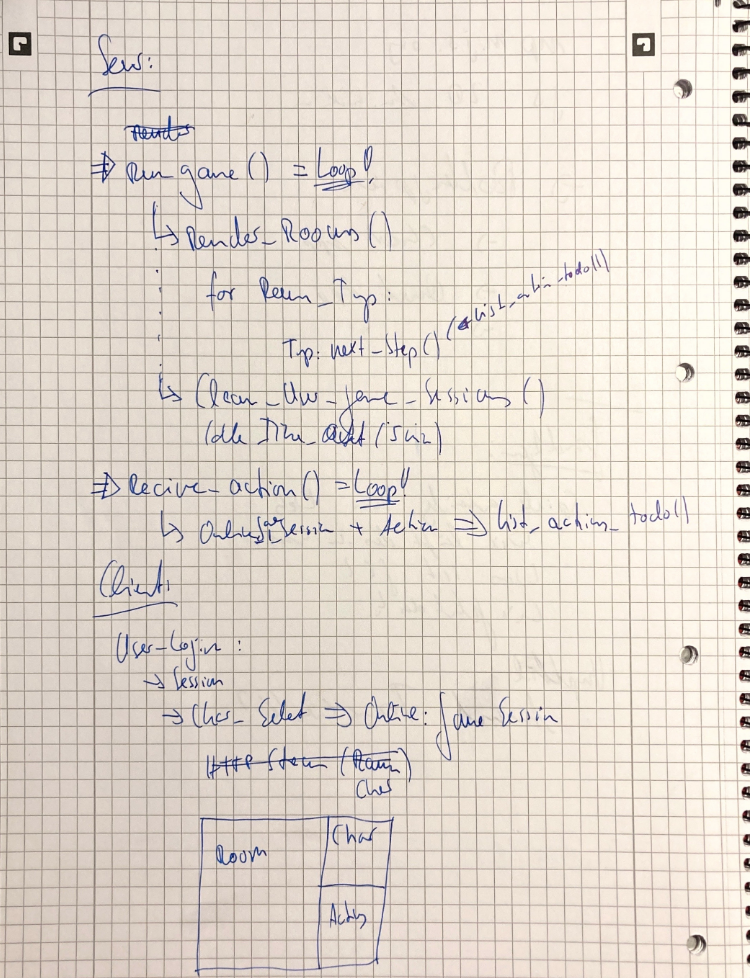
\includegraphics[width=1\textwidth]{2021-11-23-erster-entwurf-gameloop}
\end{figure}

2021-11-23-erstes-db-konzept 
\begin{figure}[H]
    \centering
    \caption[]{2021-11-23-erstes-db-konzept}
    \label{fig:2021-11-23-erstes-db-konzept}
    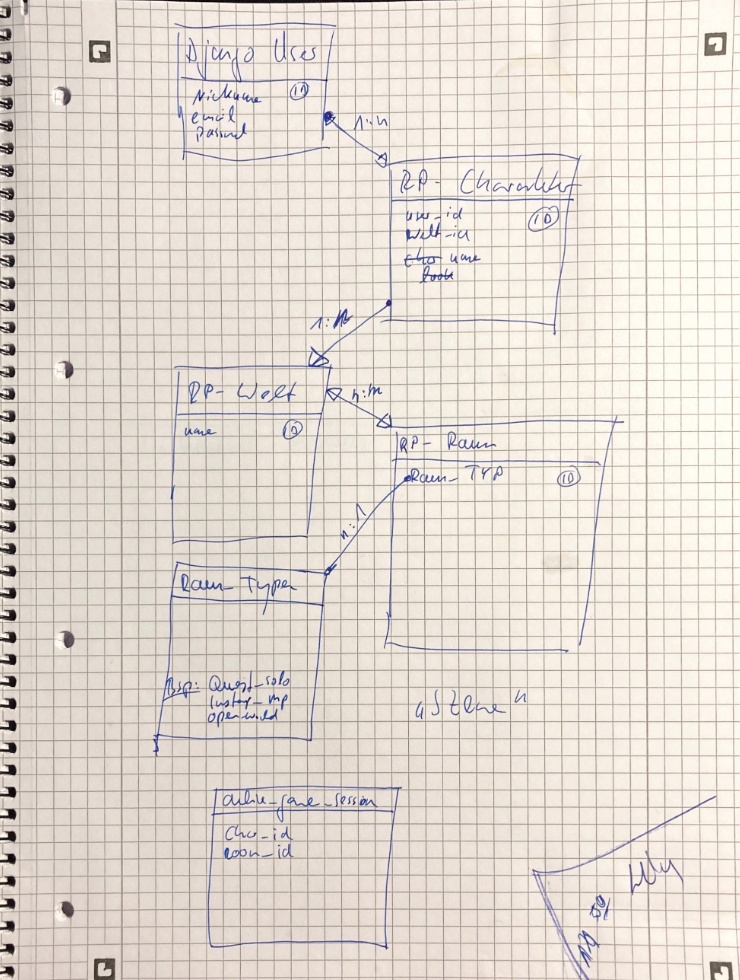
\includegraphics[width=1\textwidth]{2021-11-23-erstes-db-konzept}
\end{figure}

2021-11-27-erstentwurf-ui 
\begin{figure}[H]
    \centering
    \caption[]{2021-11-27-erstentwurf-ui}
    \label{fig:2021-11-27-erstentwurf-ui}
    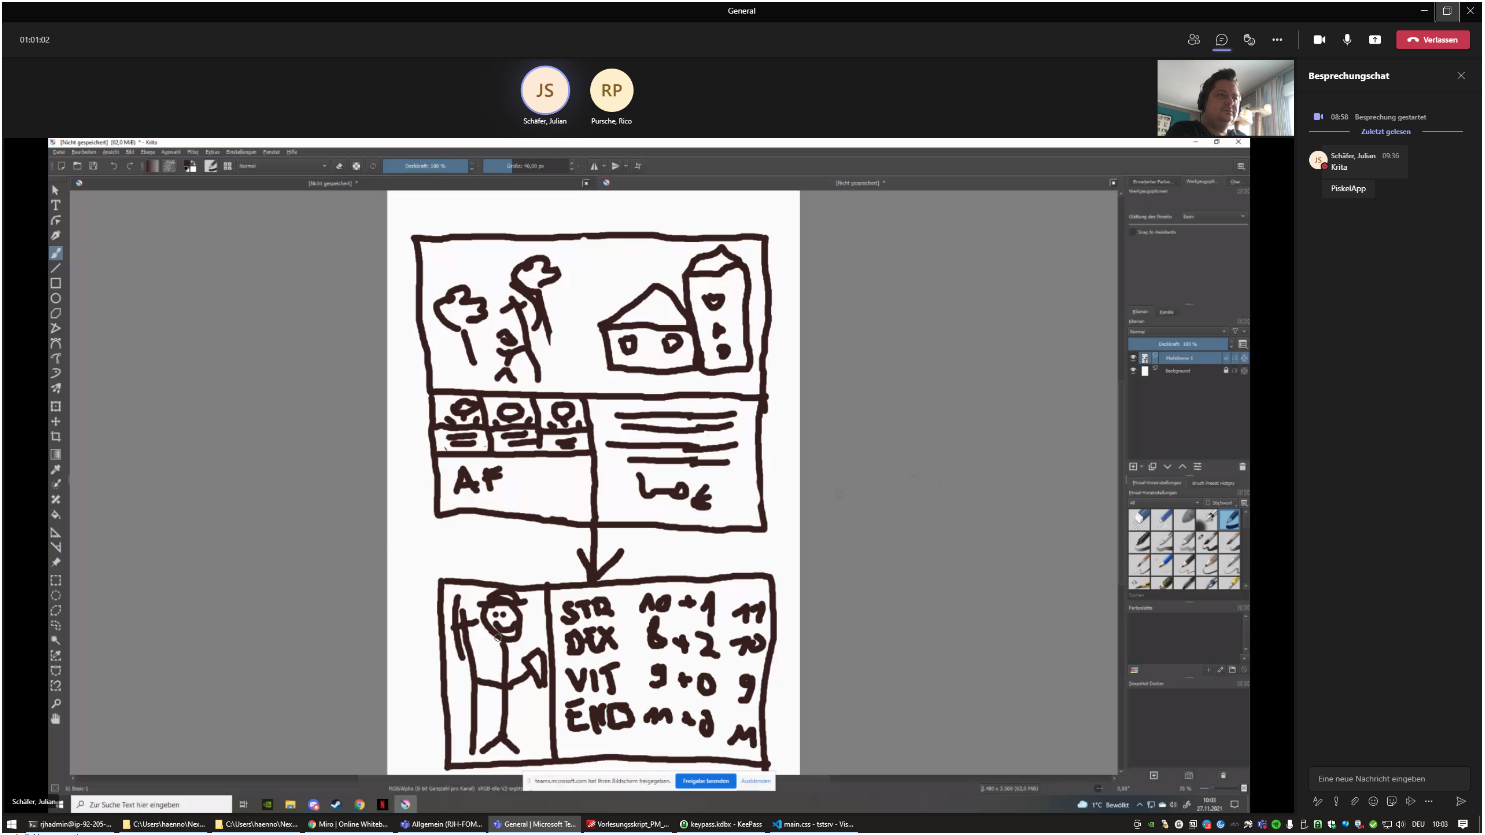
\includegraphics[width=1\textwidth]{2021-11-27-erstentwurf-ui}
\end{figure}

2021-11-27-projektskizze-1 
\begin{figure}[H]
    \centering
    \caption[]{2021-11-27-projektskizze-1}
    \label{fig:2021-11-27-projektskizze-1}
    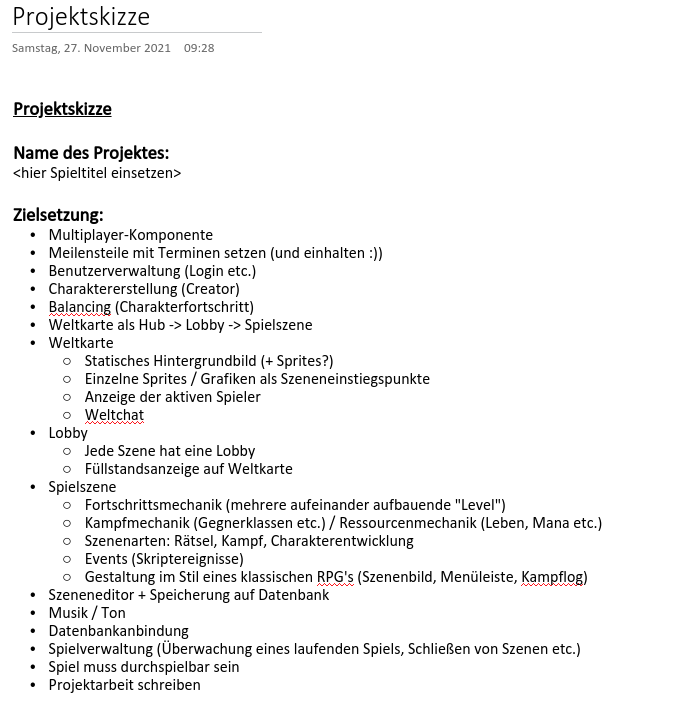
\includegraphics[width=1\textwidth]{2021-11-27-projektskizze-1}
\end{figure}

2021-11-27-projektskizze-2 
\begin{figure}[H]
    \centering
    \caption[]{2021-11-27-projektskizze-2}
    \label{fig:2021-11-27-projektskizze-2}
    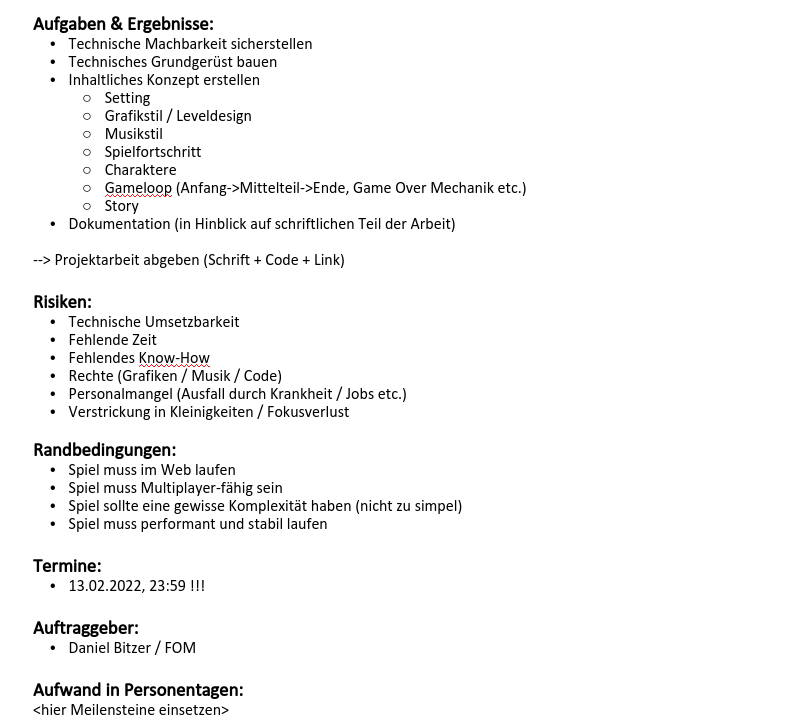
\includegraphics[width=1\textwidth]{2021-11-27-projektskizze-2}
\end{figure}

2021-11-29-Entwurf-Klassen-Ui 
\begin{figure}[H]
    \centering
    \caption[]{2021-11-29-Entwurf-Klassen-Ui}
    \label{fig:2021-11-29-Entwurf-Klassen-Ui}
    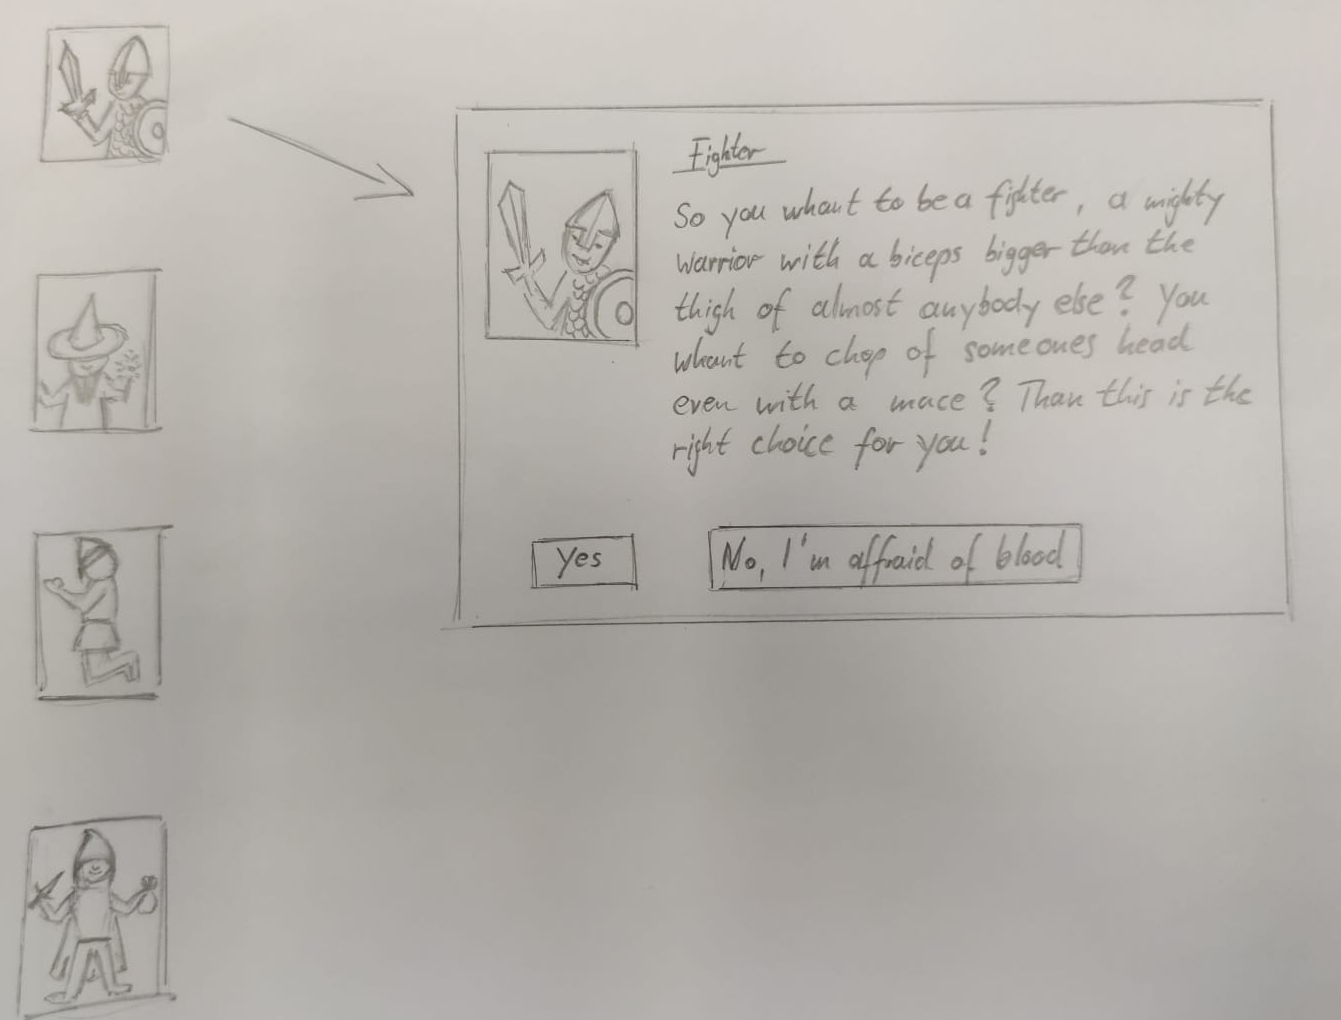
\includegraphics[width=1\textwidth]{2021-11-29-Entwurf-Klassen-Ui}
\end{figure}

2021-11-30-Entwurf-Lobby-Logik 
\begin{figure}[H]
    \centering
    \caption[]{2021-11-30-Entwurf-Lobby-Logik}
    \label{fig:2021-11-30-Entwurf-Lobby-Logik}
    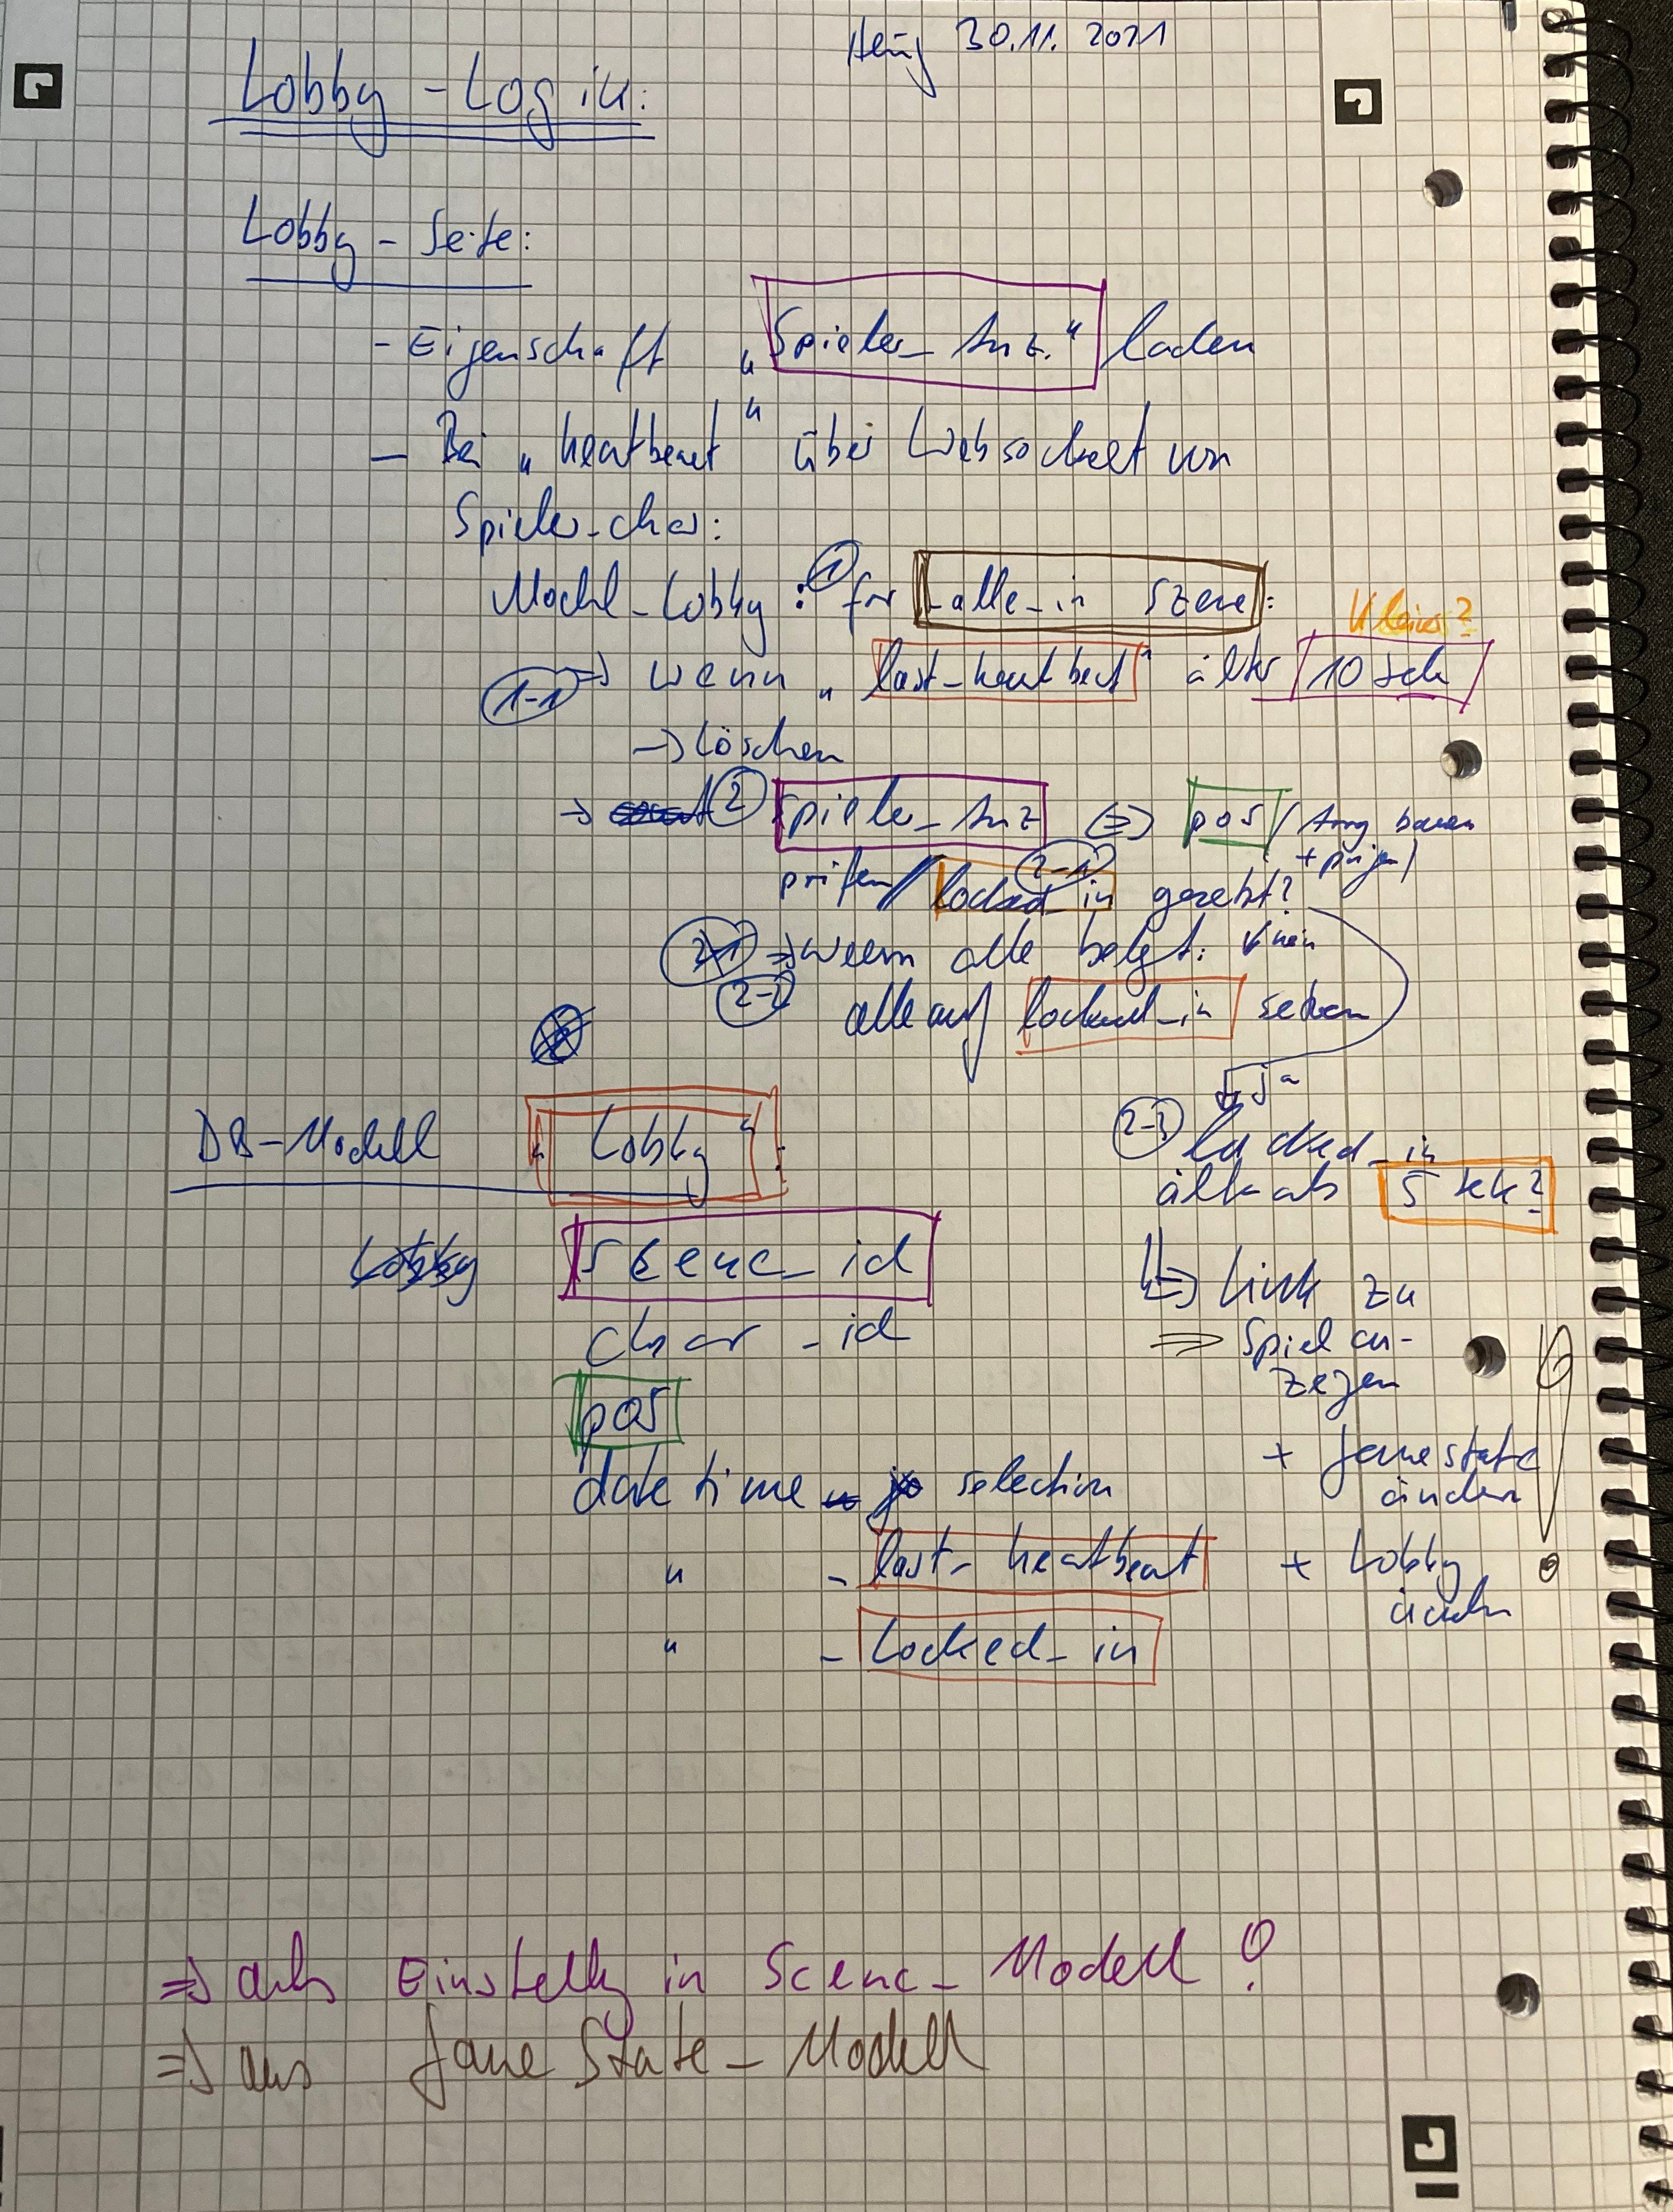
\includegraphics[width=1\textwidth]{2021-11-30-Entwurf-Lobby-Logik}
\end{figure}

2021-11-30-Entwurf-Lobby-UI 
\begin{figure}[H]
    \centering
    \caption[]{2021-11-30-Entwurf-Lobby-UI}
    \label{fig:2021-11-30-Entwurf-Lobby-UI}
    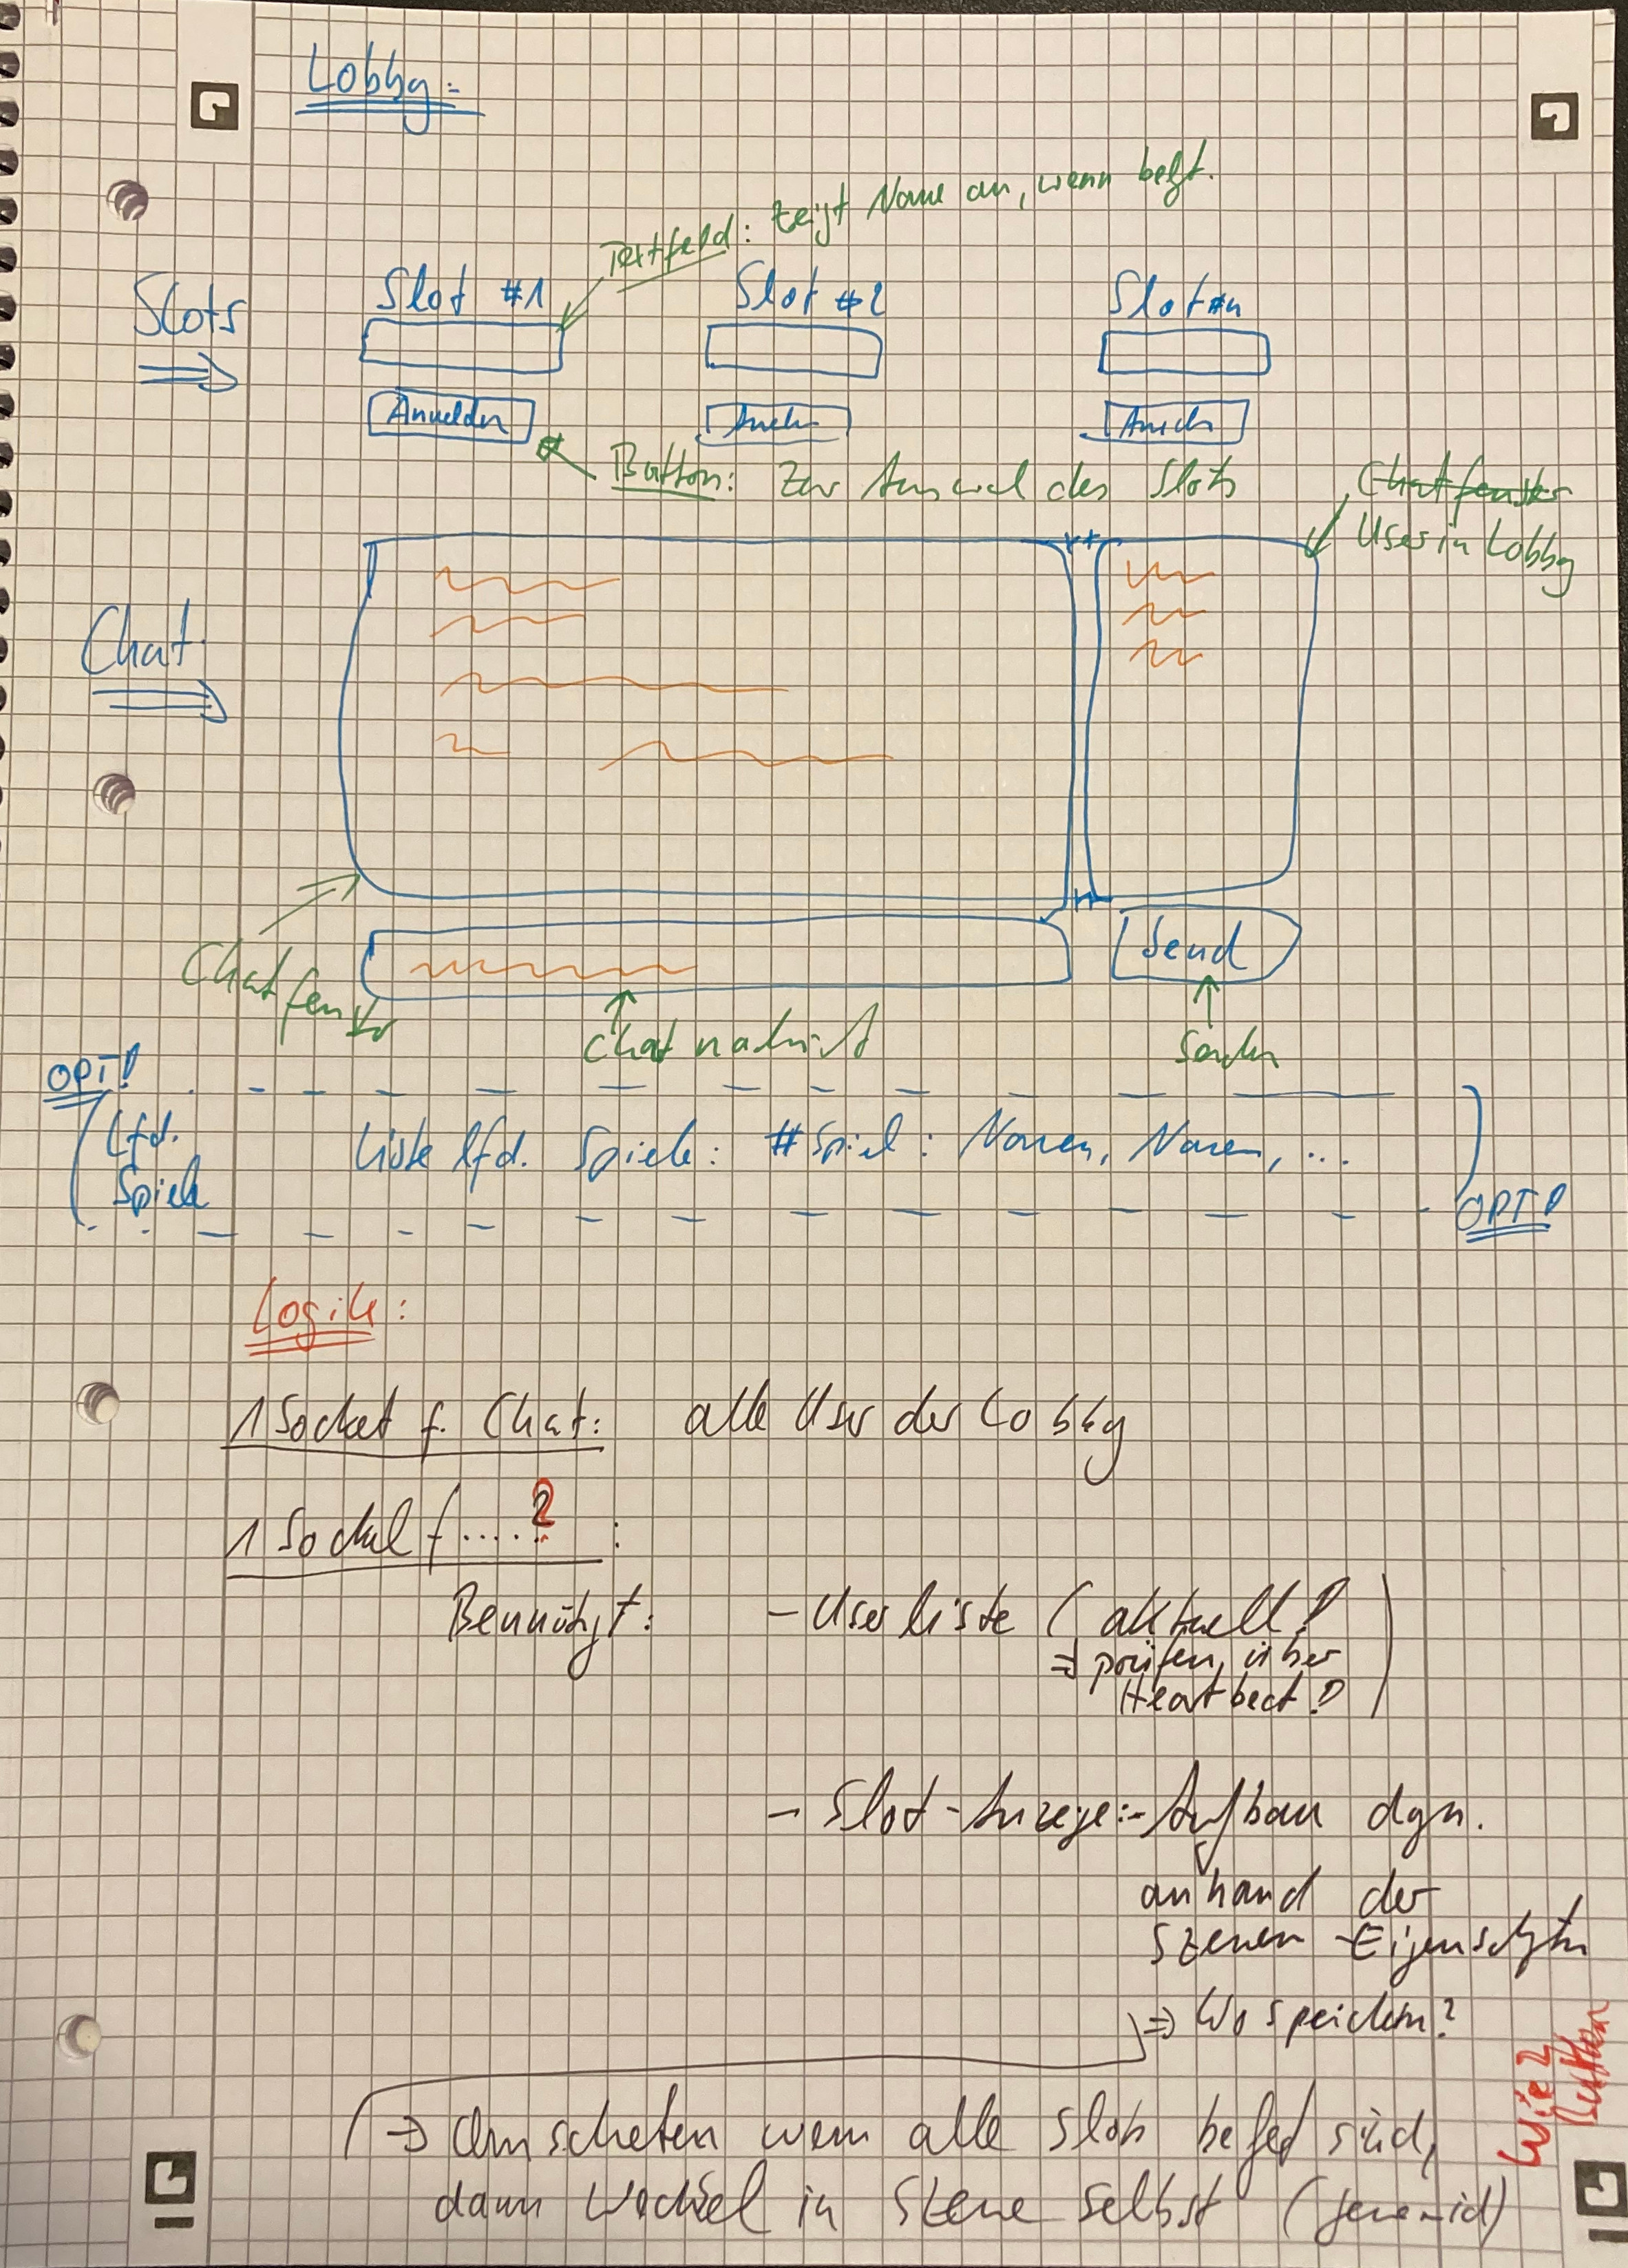
\includegraphics[width=1\textwidth]{2021-11-30-Entwurf-Lobby-UI}
\end{figure}

2021-12-02-Countdown-Logik 
\begin{figure}[H]
    \centering
    \caption[]{2021-12-02-Countdown-Logik}
    \label{fig:2021-12-02-Countdown-Logik}
    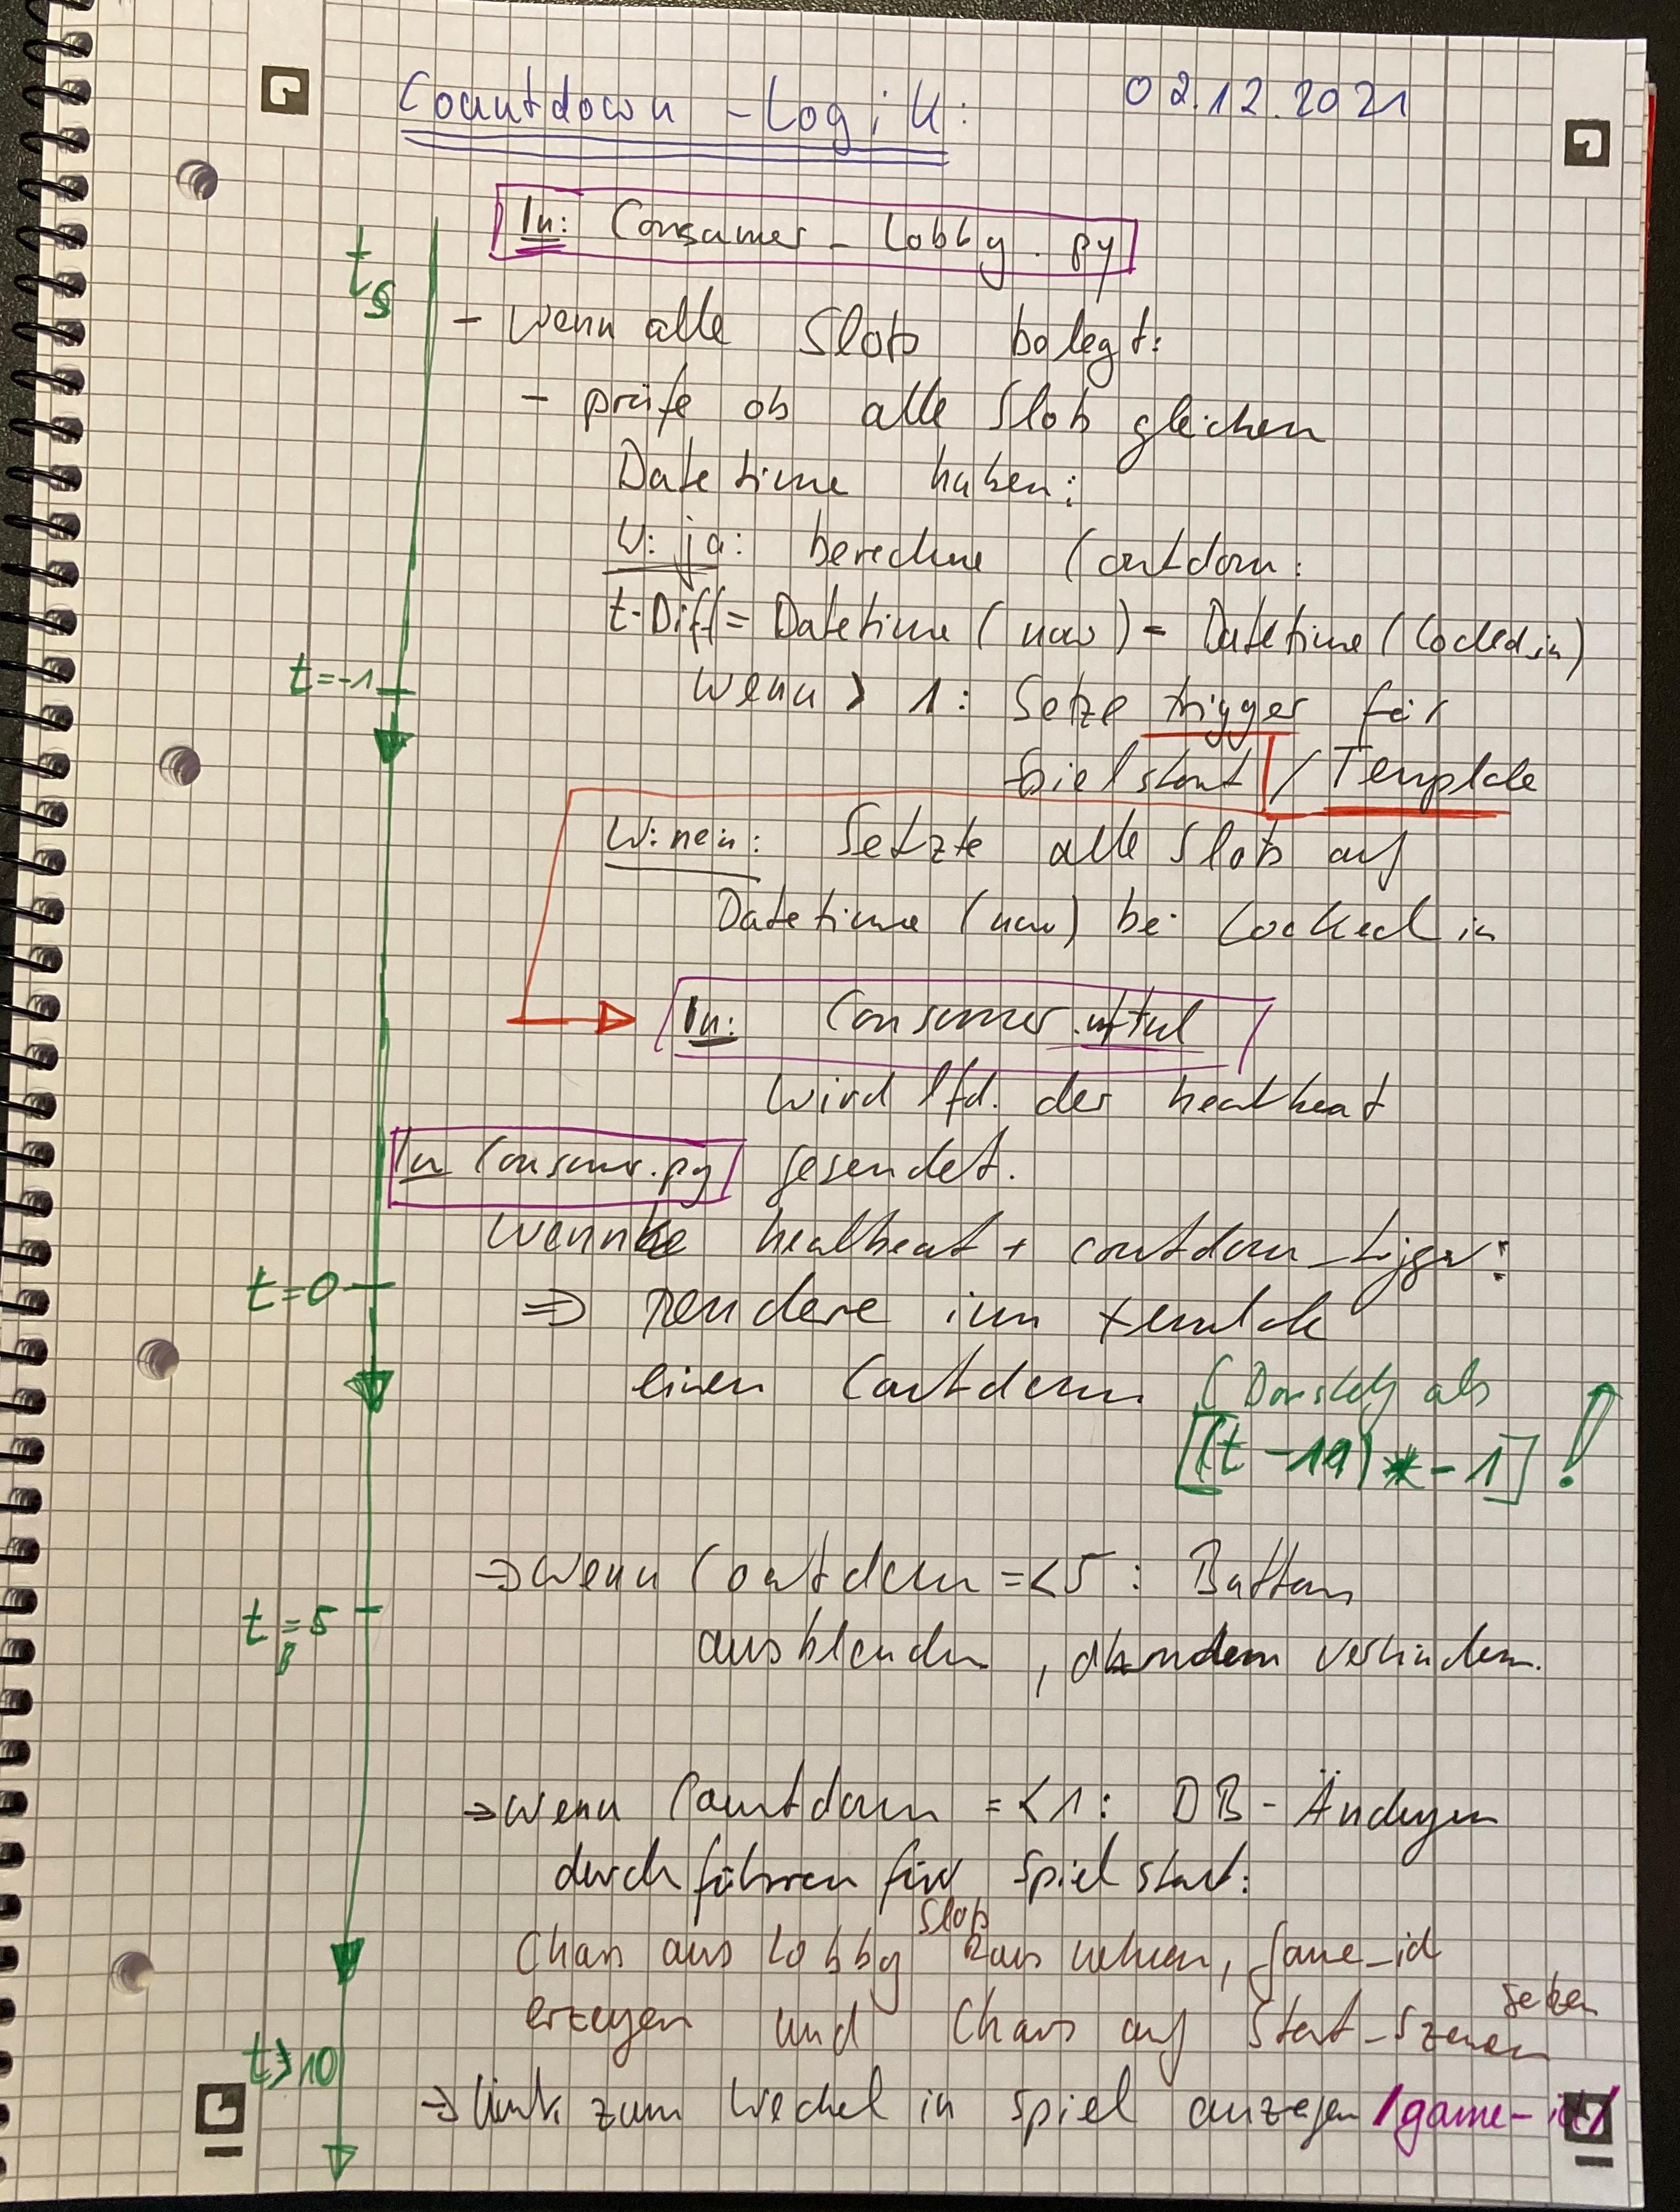
\includegraphics[width=1\textwidth]{2021-12-02-Countdown-Logik}
\end{figure}

2021-12-05-Projketbesprechung-Miro-b 
\begin{figure}[H]
    \centering
    \caption[]{2021-12-05-Projketbesprechung-Miro-b}
    \label{fig:2021-12-05-Projketbesprechung-Miro-b}
    
\includegraphics[width=1\textwidth]{2021-12-05-Projketbesprechung-Miro-b}
\end{figure}

2021-12-05-Projketbesprechung-Miro-c 
\begin{figure}[H]
    \centering
    \caption[]{2021-12-05-Projketbesprechung-Miro-c}
    \label{fig:2021-12-05-Projketbesprechung-Miro-c}
    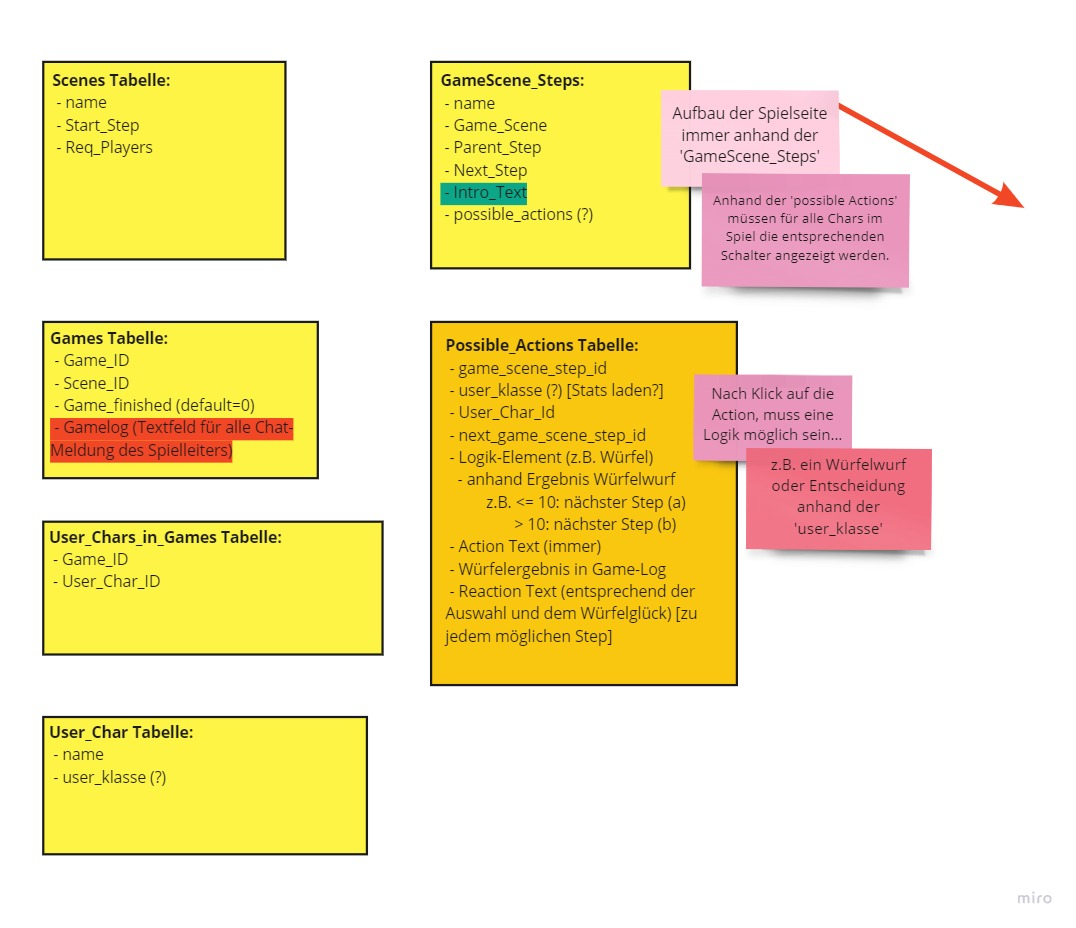
\includegraphics[width=1\textwidth]{2021-12-05-Projketbesprechung-Miro-c}
\end{figure}

2021-12-05-Projketbesprechung-Miro-d 
\begin{figure}[H]
    \centering
    \caption[]{2021-12-05-Projketbesprechung-Miro-d}
    \label{fig:2021-12-05-Projketbesprechung-Miro-d}
    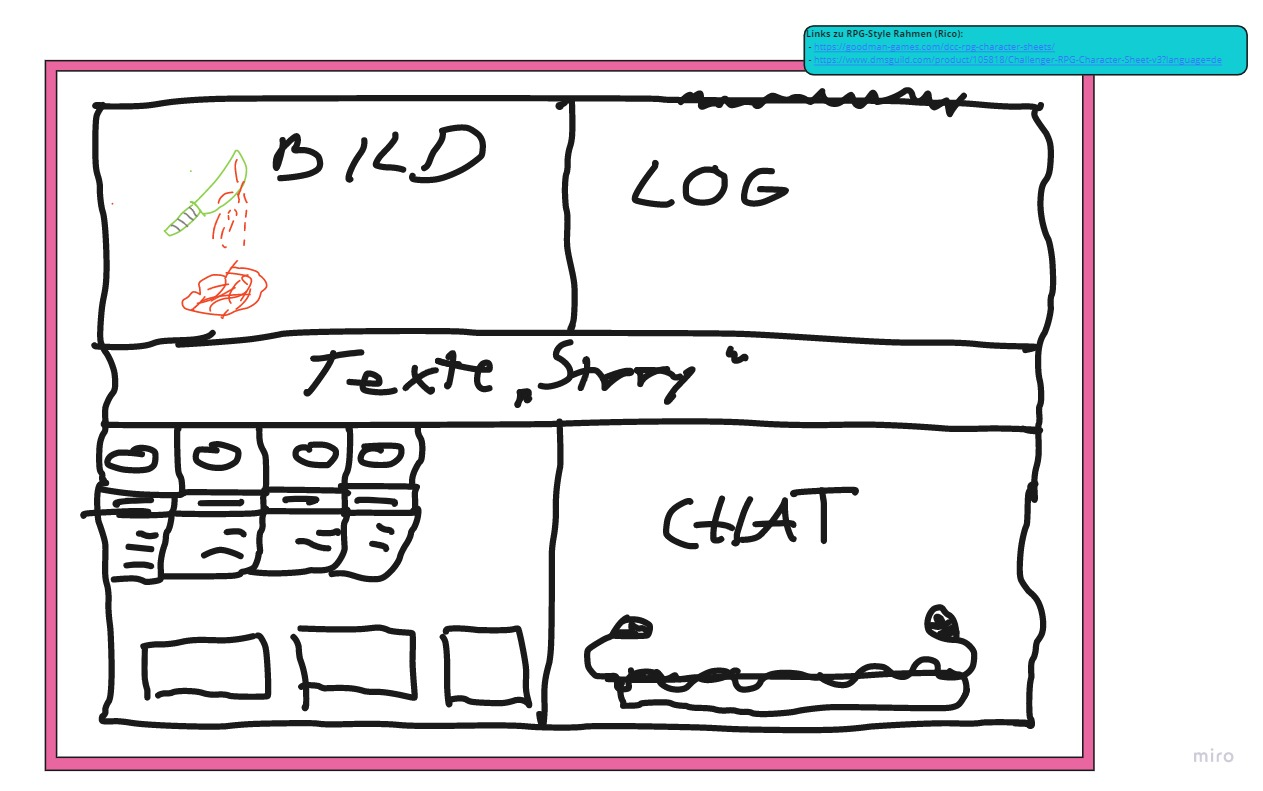
\includegraphics[width=1\textwidth]{2021-12-05-Projketbesprechung-Miro-d}
\end{figure}

2021-12-11-Projekt-Besprechung-Klassenbeschreibung 
\begin{figure}[H]
    \centering
    \caption[]{2021-12-11-Projekt-Besprechung-Klassenbeschreibung}
    \label{fig:2021-12-11-Projekt-Besprechung-Klassenbeschreibung}
    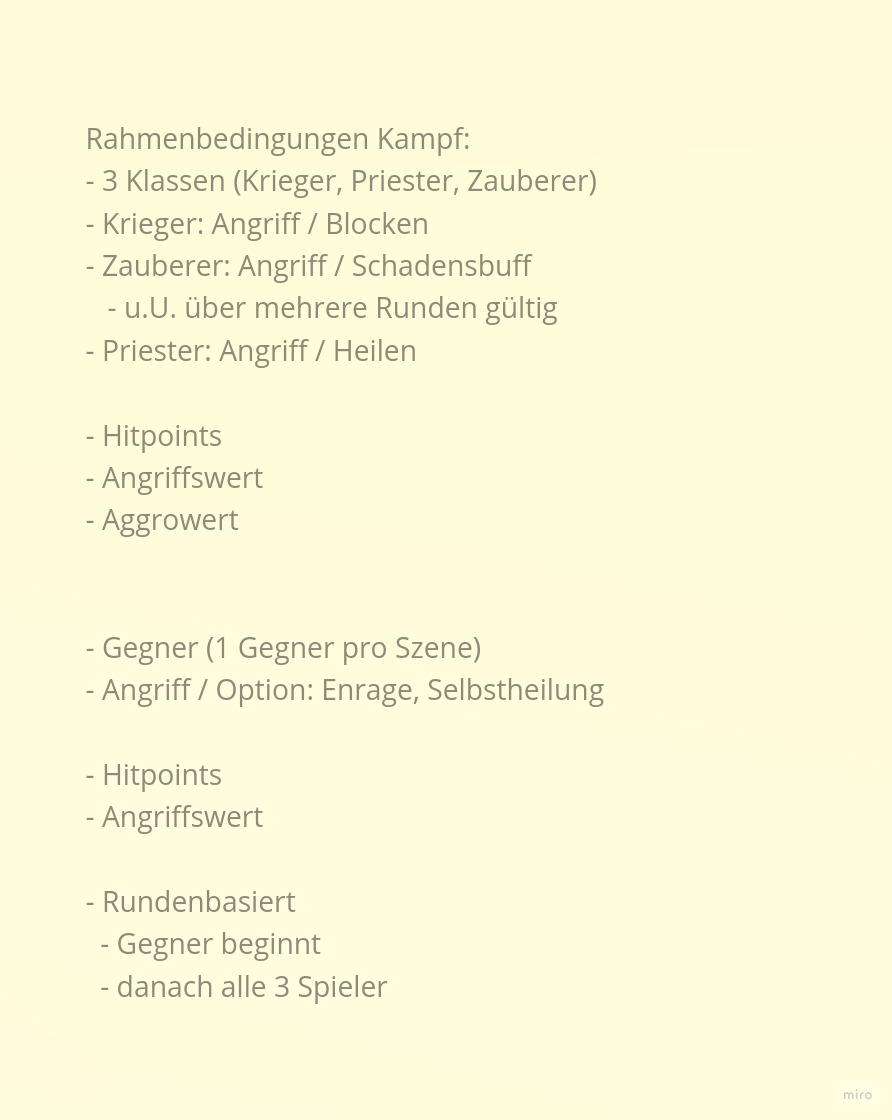
\includegraphics[width=1\textwidth]{2021-12-11-Projekt-Besprechung-Klassenbeschreibung}
\end{figure}


\begin{figure}[H]
    \centering
    \caption[]{11.12.2021: Projekt Besprechung: Gegenseitiges Update und Wechsel von Szenenlogik zu Kampfsystem für das RPG }
    \label{fig:2021-12-11-Projekt-Besprechung}
    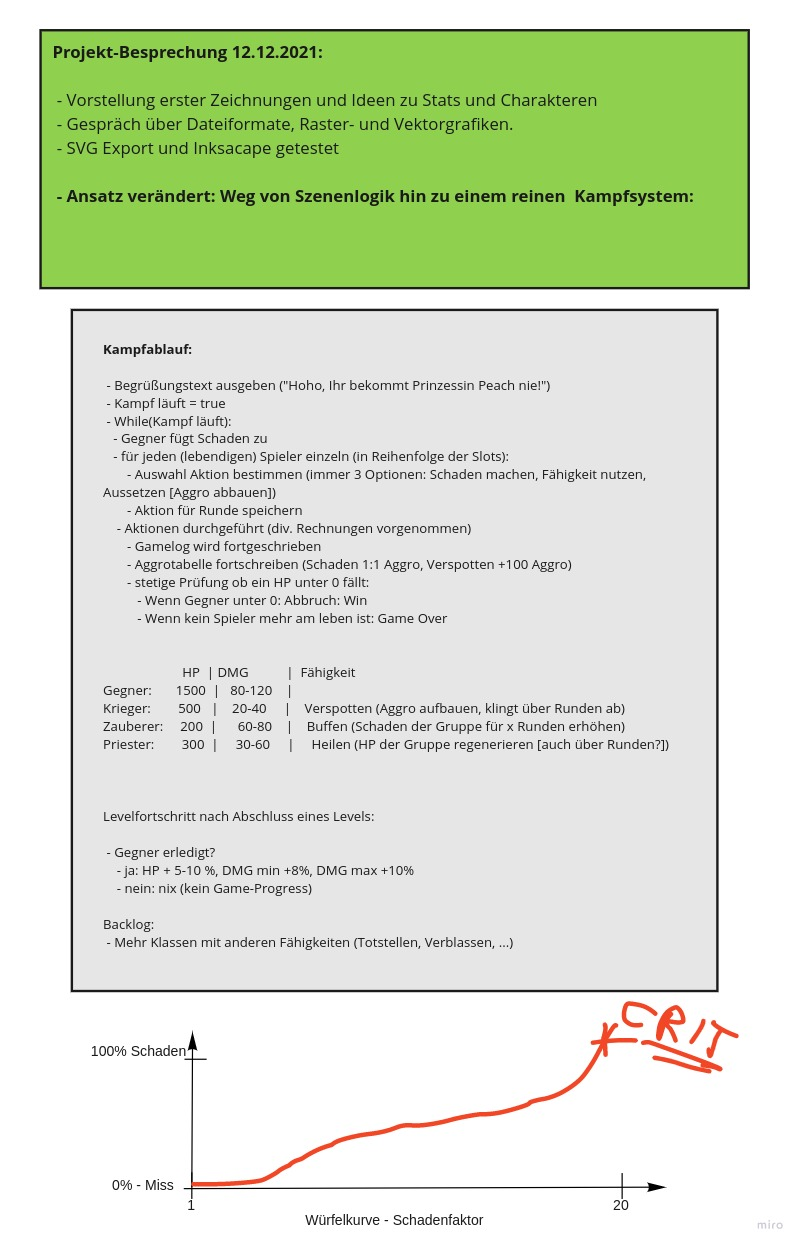
\includegraphics[width=1\textwidth]{2021-12-11-Projekt-Besprechung}
\end{figure}


\begin{figure}[H]
    \centering
    \caption[]{06.01.2022: Projekt Besprechung: Ermitteln von restlichen ToDos, Aufgabenverteilung, Meilienstein- und Terminplanung}
    \label{fig:2022-01-06-Projektbesprechung}
    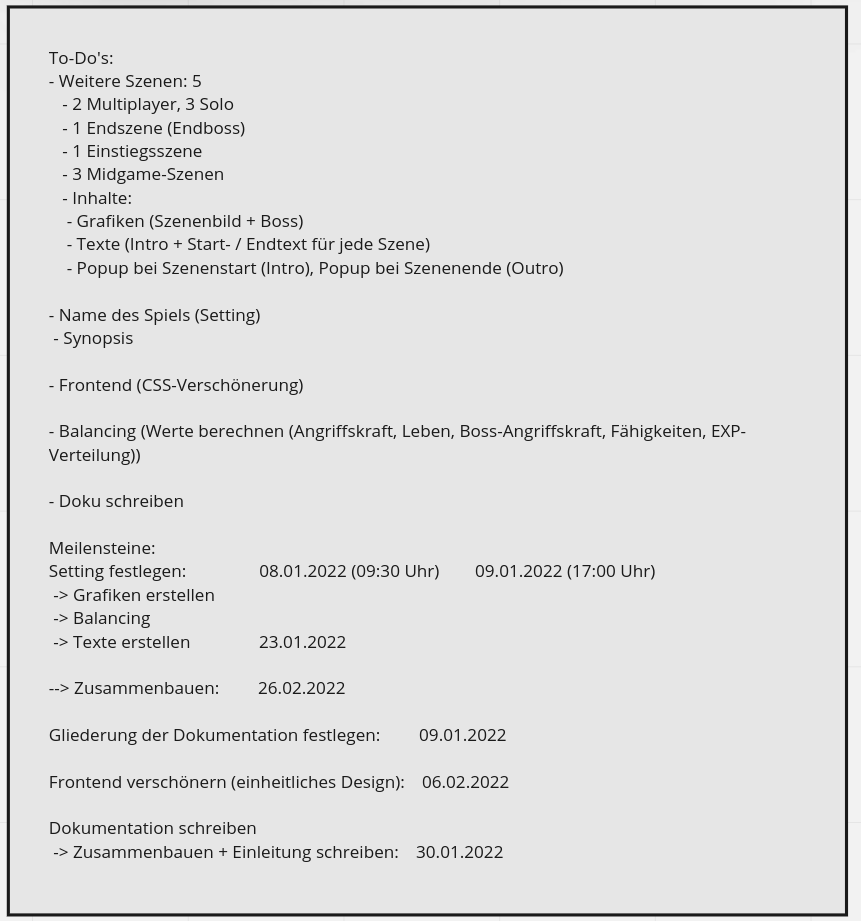
\includegraphics[width=1\textwidth]{2022-01-06-Projektbesprechung}
\end{figure}




\section{Entwicklungsnotizen}


\subsection{Entwicklung, Samstag 13.11.2021}

Allererste Tests und Anlage der Django-App sowie  hochladen des ersten Stands zu Github (Commits \url{https://git.io/JSq7n} und \url{https://git.io/JSYH4}). Eigene Notizen zum Ablauf dazu hier: 


\begin{lstlisting}
1. copy files (docker-compose, dockerfile, example.env, requirements.txt) from repo local
2. rename .env.example to .env and change settings 
3. init django with: docker-compose run rpg django-admin startproject rpg .
4. edit rpg/settings.py:
    add:
        start:
            import os
            import environ
            env = environ.Env()
            environ.Env.read_env()
        after 'BASE_DIR':
            TEMPLATES_DIR = os.path.join(BASE_DIR, 'templates')
            STATIC_DIR = os.path.join(BASE_DIR, 'static')
        after STATIC_URL:
            STATICFILES_DIRS = [
                STATIC_DIR,
            ]
    change: 
        SECRET_KEY to:
            SECRET_KEY = env('ENV_SECRET_KEY')
        ALLOWED_HOSTS to:
            ALLOWED_HOSTS = [env('ENV_ALLOWED_HOSTS')]
        in Templates, Dirs to:
                'DIRS': [TEMPLATES_DIR],
        DATABASES to:
            DATABASES = {
                'default': {
                    'ENGINE': 'django.db.backends.postgresql',
                    'NAME': env('ENV_POSTGRES_DB'),
                    'USER': env('ENV_POSTGRES_USER'),
                    'PASSWORD': env('ENV_POSTGRES_PASSWORD'),
                }
            }

5. copy and rename .env.example also to rpg/.env (remeber to copy again @changes)
6. update django to new db: 'docker-compose run python manage.py makemigrations' and 'docker-compose run python manage.py migrate'
7. create superuser: docker-compose run rpg python manage.py createsuperuser
8. create django app: docker-compose run rpg python manage.py startapp rjh_rpg 
\end{lstlisting}




\subsection{Entwicklung, Mittwoch 24.11.2021}

Einbau von Grundlagen: 
\begin{itemize}
    \item Update der Django-Basis Installtion bzw. des Projektes (Commit \url{https://git.io/JSqbt}). 
    \item Einbau der Benutzer-Anmeldung im Django-System insbesondere unter Nutzung von zwei Anleitungen   \footnote{Siehe  \url{https://www.nintyzeros.com/2020/06/login-register-user\%20page-in\%20django.html} und \url{https://docs.djangoproject.com/en/3.2/topics/auth/default/\#built-in-auth-forms}.}.
    \item Auto-Download und restart der Docker-Container bei neuen Commits im Repository auf Github per Cron-Jobjob-Script (siehe \url{https://git.io/JStjW}).
\end{itemize}




\subsection{Entwicklung, Donnerstag 25.11.2021}

Einbau der Charaktere als Datenbank-Modell und View in Django (Commit \url{https://git.io/JSmOd}).



\subsection{Entwicklung, Samstag 27.11.2021}

Einbau der Weltkarte bzw. Levelauswahl (Commit \url{https://git.io/JSmG8}).



\subsection{Entwicklung, Sonntag 28.11.2021}

\begin{itemize}
    \item Einbau einer Web-Sockets Chat-Funktion unter Nutzung einer Anleitung\footnote{Siehe \url{https://github.com/veryacademy/YT-Django-Project-Chatroom-Getting-Started}. } (Commit \url{https://git.io/JSmlS} sowie folgender Commits von diesem Tag).
    \item (Teilweise) Installation der Entwicklungsumgebung, Docker sowie Git bei Julian und Rico sowie jeweils zwei erste Test-Commits incl. anschließendem Auto-Update des Servers (Rico: \url{https://git.io/JSmKV} und Julian: \url{https://git.io/JSmoF}).
\end{itemize}



\subsection{Entwicklung, Montag 29.11.2021}

Erstellung eines Web-Sockets für eine Counter-Funktion incl. der notwendigen Anpassungen an Datenbankmodell, der Django-Reciver und -Consumer (Commit \url{https://git.io/JSmDa}).



\subsection{Entwicklung, Dienstag 30.11.2021}

Einbau einer Lobby und einer Chatfunktion in dieser Lobby -- Jeweils abhängig von der Lobby werden dynamisch Websockets geöffnet (Commits \url{https://git.io/JSm5n} und \url{https://git.io/JSm5N} sowie weitere Anpassungen und Korrekturen in den Commits vom 01.12.2021).


\subsection{Entwicklung, Samstag 04.12.2021}

Flask8 als Code-Linter genutzt und einige Anpassungen entsprechend vorgenommen (Commit \url{https://git.io/JSmN2}).


\subsection{Entwicklung, Sonntag 05.12.2021}

Einbau der Spielseite selbst als logischer Schritte nach der Weltkarte (als Levelauswahl) und der Lobby (Spielfindung /-erstellung) (Commits \url{https://git.io/JSYLS}, \url{https://git.io/JSYqd} und \url{https://git.io/JSYmV}).



\subsection{Entwicklung, Sonntag 12.12.2021:}

Als Grundlage der Dokumentation eine an APA-Zietierrichtlinien angepasste Variante der LaTeX-FOM-Vorlage\footnote{Siehe \url{https://github.com/andygrunwald/FOM-LaTeX-Template}.} in der Git-Repostitory eingefüht und für das Projekt hier angepasst. Dort erfolgt nun laufen auch die Dokumentation (Commit \url{https://git.io/JSYOZ}). 



\subsection{Entwicklung, Sonntag 19.12.2021:}

An diesem Tag wurden weitere, notwenige Grundlagen für die Integration der Spiellogik eingebaut. Das insbesondere in Vorbereitung auf die kommenden Anpassungen und Entwicklungen die in der Projektbesprechung vom 11.12.2021 besprochen wurden. 
Konkret: 

\begin{itemize}
	\item Prüfung auf den Seiten Chars, Worldmap und Lobby ob dieser Benutzer ein aktives Spiel hat. Falls ja, wird der Benutzer auf diese Seite umgeleitet.
	\item Grundfunktion für das Beenden von einem Spiel eingebaut: Man kann nun per Klick im Spiel, das Spiel beenden.
	\item Daran anschließend eine Prüfung im laufendem Spiel, ob das Spiele beendet wurde und falls ja, Anzeige eines Endbildschirms.
\end{itemize}

Die Entwicklung der Grundlagen an diesem Tag wurde mit Fokus auf Modularisierung erledigt. Der Code der jeweiligen Funktionen wurde in einzelnen Dateien ausgelagert um Wiederverwendbarkeit und Lesbarkeit zu erhöhen. 

Die zugehörigen Commits sind insbesondere: 
\url{https://git.io/JDjKl} und 
\url{https://git.io/JDjKB}


\subsection{Entwicklung, Dienstag 21.12.2021:}

Grundlagen des Kampfsystems entsprechend der Projekt-Besprechung vom 11.12.2021 (Abbildung \ref{fig:2021-12-11-Projekt-Besprechung}) sollen implementiert werden.

Vorbereitungen: 

\begin{itemize}
    \item Tabelle "GamesScenesSteps" und Verknüpfungen entfernen (Commits \url{https://git.io/JDjKz} und \url{https://git.io/JDjKg})
    \item Kampf-/Gamelog erzeugen: Darin werden alle Meldungen aus dem Spiel wie z.B. Kampftexte, Schaden, Aktionen, Systemmeldungen und alles andere denkbare angezeigt und gespeichert. Getrennt davon soll der Chat-Log dargestellt werden. Dazu werden in der Tabelle "Games" zwei neue Textfelder erzeugt (Commit \url{https://git.io/JDj63}). 
    \item Anzeige des Game-Logs auf der Spielseite. Schreiben von Nachrichten in das Gamelog als ersten Test des grundlegend umgestellten Seitenaufbaus: Es werden nur noch einzelene Elementinhalte per Websocket transportiert, nicht mehr ganze HTML-Code-Blöcke (Commit \url{https://git.io/JyeJQ}).
\end{itemize}


\subsection{Entwicklung, Montag 27.12.2021:} \label{ref-runden-impl}

Weitere Entwicklungen entsprechend der Projekt-Besprechung vom 11.12.2021 (Abbildung \ref{fig:2021-12-11-Projekt-Besprechung}):

\begin{itemize}
    \item Eintrag ins Gamelog zum Spielstart (Commit \url{https://git.io/JyBRf}).
    \item Rundensystem implementieren. Dazu mindestens notwendig: Lebens- und Angriffspunkte der User-Chars sowie des Gegners. 
    \begin{enumerate}
        \item Erster Schritt: Definition des Ablaufes einer Runde als Pseudo-Code: 
            \begin{enumerate}
                \item Gameloop-Schleife: [round-state]
                \item Aktion von Gegner ausführen (Schaden) [100]
                \item Prüfen ob User-Char tod ist (HP < 1 = Dead-Flag: True) [200]
                \item Prüfen wie viele User-Chars noch leben (n < 1 = Gameover-Flag: True, break-Gameloop-Schleife) [300]
                \item Aktionen der User-Chars aufnehmen (Entscheidung für nächste Aktion von jedem Spieler annehmen + wegspeichern) [400]
                \item Alle Aktionen der User-Chars ausführen (Aktionen laden und ausführen: Schaden, Aktion, Passen) [500]
                \item Nach jedem Spieler, prüfen ob Gegner besiegt wurde (HP < 1 = Win-Flag: True, break-Gameloop-Schleife) [immernoch 500]
                \item Rundencounter +1 [600]
                \item Gameloop-Schleife nächster Durchlauf [700, zurück zu 100]...
            \end{enumerate}
    Steuerung über "round-state" Hilfsvariable, gespeichert in Games-Tabelle (Default=0, Gameover=990, Win=995). Da der Aufruf der Spiele-Logik über den Websocket-Heartbeat der Spieler erfolgt, müssen die Arbeitsschritte sehr kleinteilig sein und diese laufend in kleinen (kleinsten?) Schritten weggepeichert werden. Möglicherweise ergibt sich ein Sync-Problem (Commit \url{https://git.io/JyRml})
    \item Zweiter Schritt: HP und AP bei User-Chars implementieren, damit AP aus "round-state 100: Gegner führt Schaden aus" durchgeführt werden kann (Commit \url{https://git.io/JyRWD}).  
    \end{enumerate}
\end{itemize}


\subsection{Entwicklung, Dienstag 28.12.2021:}

Fortführung der Entwicklungen vom Vortag. Hier insbesondere nun die Implementation der aller Funktionen der Runden- bzw. Spiellogik:

\begin{itemize}
    \item Auswahl eines zufälligen, lebenden Spielercharakters und zufügen von Schaden durch den Gegener. Außerdem Erweiterung Runden-/Gameloop und Fortschreiben des Game-Logs (Commit \url{https://git.io/JygDz}).
    \item Nächster Rundenschritt 200: Prüfen ob Spieler gestorben sind und Meldung im Game-Log ausgeben falls in aktueller Runde gestorben (Commit \url{https://git.io/Jya3H}). 
\end{itemize}


\subsection{Entwicklung, Mittwoch 29.12.2021:}

Weitere Implementation von Rundenlogik:

\begin{itemize}
    \item Rundenschritt 300: Feststellen ob alle Spieler verstorben sind, falls ja in Spielende springen (Commit \url{https://git.io/Jy1Lu}).
    \item Tests ergaben Probleme beim Spiel mit mehreren Spielern. Die Rundenlogik wird dann gleichzeitig vorangetrieben. Dadurch werden manche Aktionen und Rundenschritte mehrfach ausgeführt. Ein Versuch das Problem mit einem Token (ähnlich einem Semaphor) zu lösen, brachte leider noch keinen abschließenden Erfolg. Der Singleplayer aber, geht fehlerfrei. Das Problem wird daher zurückgestellt und nun zuerst die Entwicklung weiterer Punkte fortgeführt (Commit \url{https://git.io/Jy1qZ}).
    \item Als Workaround für oben genanntes Problem im Mulitplayer wurde nun eingestellt, dass immer nur der erste Spieler eines Spiels die Rundenlogik vorantreibt. Das ist etwas mehr fehleranfällig als eine korrekte Tokenlösung, wird für das Projekt hier aber vorerst ausreichend sein (Commit \url{https://git.io/Jy1su}).
    \item Umfangreiche Erweiterungen und Anpassungen für das Anzeigen der User-Chars auf der Spieleseite, darstellen und aussteuern der Aktions-Buttons, das einsammeln der Aktionen in der Datenbank und ebenso bereits das zurücksetzen beim Rundenwechsel (Commit \url{https://git.io/JyDlp}).

    \begin{figure}[H]
        \centering
        \caption[]{29.12.2021: Bildschirmfoto zum Entwicklungsstand mit Runden-Status 400.}
        \label{fig:2021-12-29-Bildschirmfoto-Entwicklungsstand-Runden-Status-400.png}
        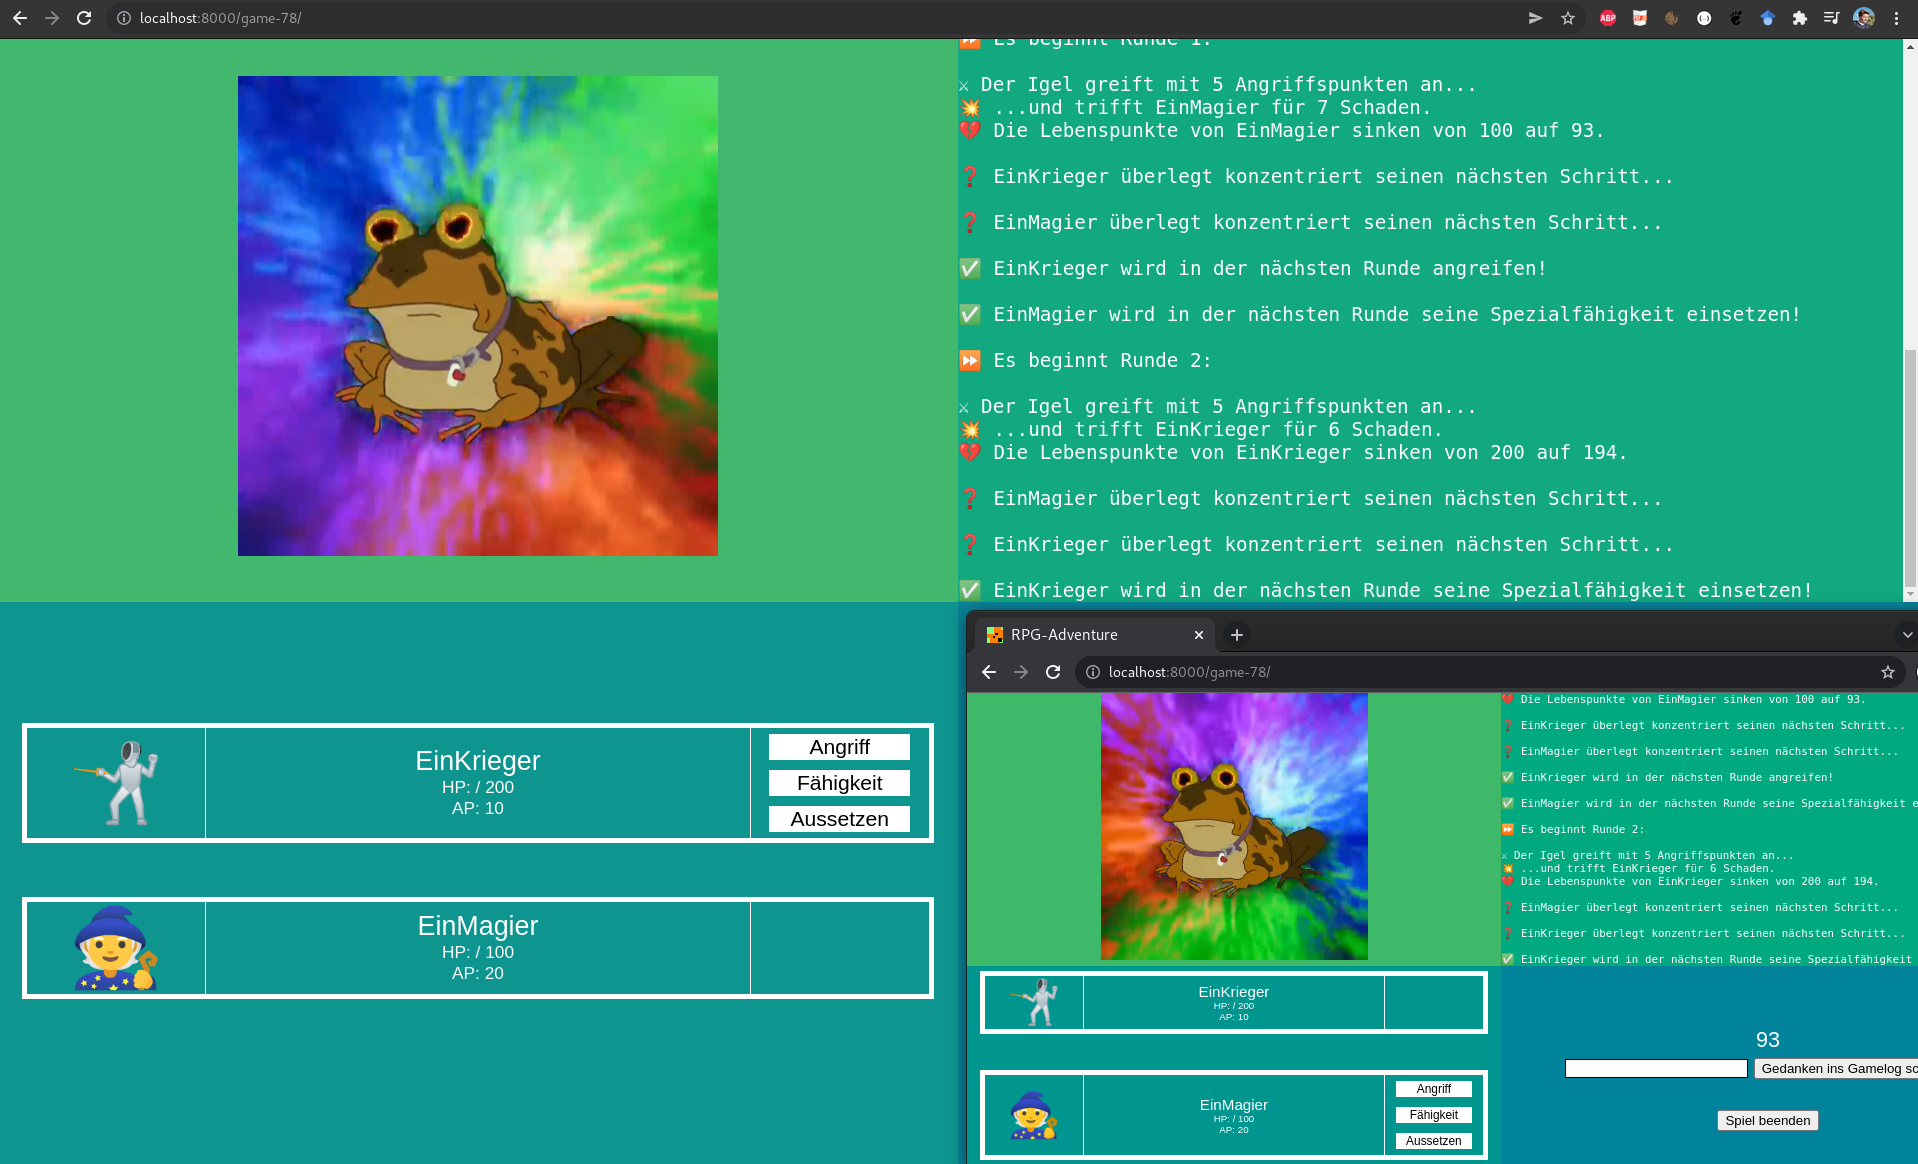
\includegraphics[width=0.7\textwidth]{2021-12-29-Bildschirmfoto-Entwicklungsstand-Runden-Status-400.png}
    \end{figure}

    \item Die Chatfunktion wurde implementiert. Hier jedoch abweichend vom Plan direkt als Meldungen im Game-Log und nicht in einem gesonderten Chat-Log und Chat-Fenster. Julian war damit im kurzen Teams-Gespräch gestern einverstanden. Den Aufbau der Game-Seite entsprechend angepasst und dem Game-Log deutlich mehr Raum eingeräumt. Außerdem weitere Anpassungen am Design und Style (Commit \url{https://git.io/JyDRK}).

\end{itemize}


\subsection{Entwicklung, Donnerstag 30.12.2021:}

Abschließender Schritt in der Implementation der Rundenlogik:

\begin{itemize}
    \item Die Schadensfunktion für Spieler wurde eingebaut: Damit kann dem Gegner nun Schaden zugefügt werden. Außerdem Prüfung auf Tod des Gegners incl. entsprechender Medlung (Commit \url{https://git.io/Jy9E7}).
\end{itemize}

Offen sind nun als nächste Schritte noch:
\begin{enumerate}
    \item Fähigkeiten der Spieler in Rundenlogik implementieren.
    \item Abschlussbildschirm für Sieg und Gameover konzeptionieren und implementieren. 
    \item Charakterentwicklung bei Sieg implementieren.
    \item Erweiterung der Infrastruktur aus Scripten, Anleitungen und des Git-Repos hin zum laden eines Default-Datensatzes (JSON-Datei) mit nutzbaren Spieldaten (insbesondere für Testzwecke und Nutzungen durch Dritte).
\end{enumerate}


\subsection{Entwicklung, Freitag 31.12.2021:}

Abarbeiten der zuletzt genannten, nächsten Schirtte. Hier: 

\begin{itemize}
    \item Die Charakterentwicklung wird mit Erfahrungspunkten gelöst: Durch Aktionen im Spiel bzw. Kampf (Schaden bekmmen, Schaden austeilen, Fähigkeiten nutzen) bekommen die entsprechenden Charaktere sofort entsprechende Erfahrungspunkte gutgeschrieben. Wird das Spiel gewonnen, werden alle von allen teilnehmenden Spielern in dieser Runde erspielten Erfarungspunkte noch einmal verdoppelt und jedem der Spieler gutgeschrieben. Verwendet werden können diese Erfahrungspunkte dann in der Charakteransicht um damit z.B. Lebenspunkte (HP) oder Angriffspunkte (AP) zu erhöhen (Commit \url{https://git.io/Jy7gl}).
\end{itemize}


\subsection{Entwicklung, Samstag 01.01.2022:}

Nach kurzer Abstimmung und Vorstellung meiner Ergebnisse bei Julian, letzte Anpassungen bzw. Entwicklungen: 

\begin{itemize}
    \item Ausgabe der erhaltenen XP beschleunigt: Es werden nun immer 10\% (aufgrundet auf die nächste Ganzzahl) der XP ausgegeben (Commit \url{https://git.io/JSTIq}).
    \item Einbau der Charakter-Fähigkeiten (Commit \url{https://git.io/JSkKJ}):
    \begin{itemize}
        \item Priester: Gruppe heilen=Alle HP erhöhen
        \item Zauberer: Schaden der Gruppe erhöhen=Alle AP erhöhen
        \item Krieger: Gegner blocken=AP Gegner verringern
    \end{itemize} 
    Damit die Fähigkeiten über mehrere Runden wirken können, musste eine Hilfstabelle angelegt werden: "AbilitysToApply". Hieraus werden zum Rundenwechsel die jeweils anzuwendenden Fähigkeiten gelesen und auf die relevaten Zahlen gewirkt. 
    \item Beispieldaten hinzugefügt und automatisches laden in die Datenbank über die local/dev-Skripte eingefügt (Commit \url{https://github.com/tstsrv-de/rpg/commit/1bfa99e89ddf2dbe817bdee2c870d1ddbe4f23c1}).
\end{itemize} 


\subsection{Entwicklung, Sonntag 02.01.2022}

Ein kurzer Anwendungstest mit einem versierten RPG-Spieler und IT-affinen Nutzer. Notizen dazu: 

\begin{itemize}
    \item Hinweis beim betreten der Lobby, dass das Spiel erst startet, wenn man einen "Platz-belegt" hat: Sofort erledigt!. 
    \item Man versuchte die Interaktion mit dem Spiel per Textkommandos über die Chatzeiel. Ineteresannte Alternative zur Nutzng der Buttons: Üübertragen in Ausblick(\ref{ausblick}). 
    \item Der erste Level ist mit über 10 Runden deutlich zu lang und muss verkürzt werden: Sofort erledigt!
\end{itemize}

Weiter wurden alle im Code enthaltenen Variablen und Konstanten in die Datenbank ausgelagtert. Dazu wurde eine neue Tabelle "MyRpgConfig" angelegt, alle Werte dorthin transportiert und im Code enstprechende Abfragen sowie weitergehende Anpassungen (z.B. Schleifen x-Fach durchlaufen) vorgenommen. Auch wurden die Beispiel- bzw. nun Basisdaten für die Datenbank entsprechend erweitert (Commits \url{https://git.io/JSGJD} und \url{https://git.io/JSGJ7}).



\section{Noitzen für Reflektion}

\subsection{Rundenbasierter vs. chaotischer Spielablauf}

Der Ansatz die Entwicklung durch den Einsatz eines rundenbasierten Ablaufs bzw. Kampfsystems deutlich zu vereinfachen, muss wohl nach den Entwicklungen vom 27.12.2021 (\ref{ref-runden-impl}) zumindest angezweifelt werden. Denn der Aufwand, der durch die dadurf notwendige Konzeptionierung und Detailplanung entsteht ist nicht zu unterschätzen. Demengegen stünde bei einem chaotischen Spielablauf lediglich das Handling der Events. 

\subsection{Kleinteilige Aufgabenpakete} 

In der Entwicklung eine überschaubare Anzahl an kleinteiligen bzw. Teilufgaben vor sich zu haben, empfinde ich als sehr hilfreich. Man hat damit einen Überblick über die Arbeit der nächsten Tage. Bei der Entwicklung der Rundenlogik hatte ich durch die Kenntniss um die nächsten Runden-Schritte hier einen guten Überblick. Der Abschluss jeder einzelnen Teil-Aufgabe sorgte da laufend für postive Motivation. 
Ich vermute, dass dieser Effekt sehr ähnlich bei den agilen Methoden zum tragen kommt und zur Motivation genutzt wird. 

\subsection{Stichwortsammlung für Refektion}

\begin{itemize}
    \item Projektaufteilung: So abstimmen, dass verschiedene Arbeitsschritte gleichzeitig von verschiedenen Personen bearbeitet werden können.  
    \item Lernkurve und Codequalität: Eigentlich müsste man am Ende eines Projektes stets noch einmal von Vorne anfangen. Allein um alles zu korrigieren bzw. anzupassen, was im Projektverlauf gelernt wurde.
\end{itemize}


\section{Ideen für Erweiterungen über diese Projektarbeit hinaus (Ausblick)} \label{ausblick}

Da der Umfang dieser Projekt beschränkt ist, können nicht alle erdachten Funktionen umgesetzt werden. Einige Ideen, sollen aber nicht ungenannt bleiben: 
\begin{enumerate}
    \item Würfel bei Schaden bzw. Angriff implementieren.
    \item Aggrotabelle und verbundene Funktionen implementieren.
    \item Inaktive und getrennte Spieler bzw. Nutzer aus den Chatfunktionen der Weltkarte und Lobby entfernen. Ggfls. auch einen Timer für das Spiel anlegen der anderen Spielern anzeigt, wenn ein Spieler inaktiv bzw. getrennt vom Server ist. 
    \item E-Mail Funktion von Django konfigurien, damit das Zurücksetzen von Passwörtern u.A. möglich wird.
\end{enumerate}

